\section{Các Biến thể và Cải tiến: Swin Transformer và DeiT}
\label{sec:vit_variants_and_improvements}

Sự ra đời của Vision Transformer (ViT) đã mở ra một chân trời mới, nhưng cũng đồng thời đặt ra những thách thức lớn. Mặc dù chứng minh được tiềm năng vượt qua CNN, ViT thuần túy bộc lộ hai điểm yếu cốt lõi đã cản trở việc áp dụng rộng rãi nó:
\begin{enumerate}
	\item \textbf{Đói dữ liệu (Data-Hungry):} Do thiếu các thiên kiến quy nạp (inductive biases) về không gian như CNN, ViT đòi hỏi việc huấn luyện trước (pre-training) trên các bộ dữ liệu quy mô cực lớn (ví dụ, JFT-300M với 300 triệu ảnh) để có thể học được các quy luật thị giác cơ bản và đạt hiệu năng cao. Khi huấn luyện từ đầu trên các bộ dữ liệu cỡ vừa như ImageNet-1K, hiệu năng của nó thường thua kém các mạng ResNet tương đương.
	\item \textbf{Thiếu cấu trúc phân cấp (Lack of Hierarchy):} ViT tạo ra các token có cùng độ phân giải không gian ở tất cả các lớp. Cấu trúc "phẳng" này không phù hợp với các tác vụ thị giác dày đặc (dense prediction tasks) như phát hiện vật thể hay phân đoạn ảnh, vốn được hưởng lợi rất nhiều từ các bản đồ đặc trưng đa tỷ lệ (multi-scale feature maps) do CNN tạo ra.
\end{enumerate}
Để giải quyết những vấn đề này, một làn sóng các kiến trúc Transformer cải tiến đã ra đời, tập trung vào việc làm cho Transformer trở nên hiệu quả hơn về dữ liệu, hiệu quả hơn về tính toán, và linh hoạt hơn cho nhiều tác vụ. Trong phần này, chúng ta sẽ khám phá hai trong số những biến thể có ảnh hưởng nhất: DeiT và Swin Transformer.

\subsection{Distillation Token: Mở rộng trực tiếp của ViT}
\label{subsubsec:deit_distillation_token}

Để khai thác tối đa lợi ích của chưng cất tri thức, DeiT không chỉ thay đổi hàm mất mát, mà còn \textbf{tích hợp trực tiếp cơ chế distillation vào kiến trúc Transformer}. Thành phần then chốt cho mục tiêu này là \textbf{Distillation Token}.

\paragraph{Mở rộng chuỗi đầu vào}

Trong Vision Transformer (ViT) tiêu chuẩn, chuỗi đầu vào có dạng:

\[
[\text{CLS}], x_1, x_2, \dots, x_N
\]

Trong DeiT, một token đặc biệt thứ hai được thêm vào:

\[
[\text{CLS}], [\text{DIST}], x_1, x_2, \dots, x_N
\]

\begin{itemize}
	\item \textbf{[CLS] token}: giữ vai trò như trong ViT, học biểu diễn phục vụ phân loại từ nhãn thật.
	\item \textbf{[DIST] token}: một token mới, được thiết kế để học trực tiếp từ mô hình giáo viên.
\end{itemize}

Hai token này được đưa qua toàn bộ Transformer encoder:
\begin{itemize}
	\item cùng tham gia self-attention
	\item cùng tương tác với tất cả patch tokens
\end{itemize}

\begin{mdframed}[style=infobox]
	\textbf{Insight}
	
	[CLS] và [DIST] không phải là hai thành phần độc lập, mà cùng chia sẻ một không gian biểu diễn và trao đổi thông tin thông qua attention.
\end{mdframed}

---

\paragraph{Hai nhánh phân loại (Two-head architecture)}

Sau khi đi qua Transformer, ta thu được hai vector đặc trưng:

\[
z_{\text{CLS}}, \quad z_{\text{DIST}}
\]

Điểm quan trọng là:

\begin{center}
	\textit{Hai vector này không dùng chung một classifier, mà đi qua hai head riêng biệt.}
\end{center}

\[
\hat{y}_{\text{CLS}} = \text{Head}_{\text{CLS}}(z_{\text{CLS}})
\]
\[
\hat{y}_{\text{DIST}} = \text{Head}_{\text{DIST}}(z_{\text{DIST}})
\]

\begin{mdframed}[style=infobox]
	\textbf{Ý nghĩa}
	
	DeiT thực chất huấn luyện \textbf{hai bộ phân loại song song}:  
	một học từ dữ liệu thật, một học từ mô hình giáo viên.
\end{mdframed}

---

\paragraph{Hai mục tiêu học khác nhau}

Hai nhánh này được tối ưu bằng hai loại tín hiệu khác nhau:

\begin{itemize}
	\item \textbf{Nhánh [CLS] (học từ dữ liệu thật):}
	\[
	\mathcal{L}_{\text{CE}}(\hat{y}_{\text{CLS}}, y_{\text{true}})
	\]
	
	\item \textbf{Nhánh [DIST] (học từ giáo viên):}
	\[
	\mathcal{L}_{\text{KL}}(\hat{y}_{\text{DIST}}, y_{\text{teacher}})
	\]
\end{itemize}

Trong đó:
\begin{itemize}
	\item $y_{\text{true}}$ là nhãn thật (one-hot)
	\item $y_{\text{teacher}}$ là phân bố xác suất từ mô hình CNN giáo viên
\end{itemize}

Tổng hàm mất mát:

\[
\mathcal{L} = (1-\alpha)\,\mathcal{L}_{\text{CE}} + \alpha\,\tau^2\,\mathcal{L}_{\text{KL}}
\]

\begin{mdframed}[style=infobox]
	\textbf{Diễn giải}
	
	[CLS] học "đáp án đúng", còn [DIST] học "cách mà một mô hình mạnh đưa ra đáp án".
\end{mdframed}

---

\paragraph{So sánh với Distillation truyền thống}

Trong các phương pháp distillation cổ điển:

\begin{itemize}
	\item Chỉ có một output duy nhất
	\item Mô hình phải học đồng thời từ hard label và soft label trên cùng một vector
\end{itemize}

Trong DeiT:

\begin{itemize}
	\item Tách thành \textbf{hai không gian học riêng biệt}
	\item Giảm xung đột giữa hai mục tiêu tối ưu
	\item Cho phép Transformer tự học cách kết hợp thông tin qua attention
\end{itemize}

\begin{mdframed}[style=infobox]
	\textbf{Insight sâu}
	
	Distillation token biến distillation từ một kỹ thuật ở mức hàm mất mát thành một \textbf{thành phần kiến trúc bên trong mô hình}.
\end{mdframed}

---

\paragraph{Giai đoạn suy luận}

Sau khi huấn luyện, ta có hai dự đoán:

\[
\hat{y}_{\text{CLS}}, \quad \hat{y}_{\text{DIST}}
\]

Có hai cách sử dụng:

\begin{itemize}
	\item Chỉ dùng $\hat{y}_{\text{CLS}}$ (giống ViT)
	\item Hoặc kết hợp:
	\[
	\hat{y} = \frac{1}{2}(\hat{y}_{\text{CLS}} + \hat{y}_{\text{DIST}})
	\]
\end{itemize}

Trong thực nghiệm, việc \textbf{trung bình hai đầu ra} thường cải thiện độ chính xác.

---

\begin{center}
	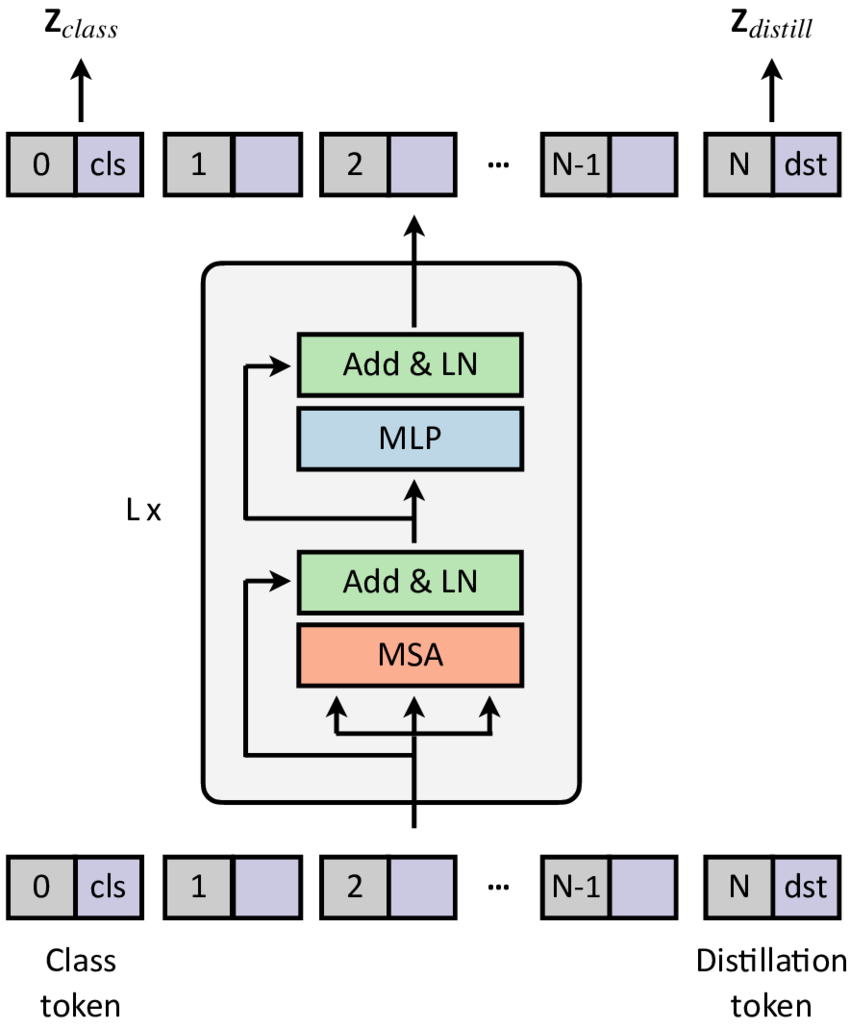
\includegraphics[width=0.9\textwidth]{images/deit_distillation_diagram.png}
	\captionof{figure}{Cơ chế distillation trong DeiT. Hai token đặc biệt ([CLS] và [DIST]) đi qua cùng Transformer nhưng được tối ưu bởi hai mục tiêu khác nhau: một từ nhãn thật và một từ mô hình giáo viên CNN.}
	\label{fig:deit_distillation}
\end{center}

\subsubsection{Kết quả và Tầm ảnh hưởng}
DeiT đã đạt được kết quả mang tính bước ngoặt: \textbf{DeiT-Base}, chỉ huấn luyện trên ImageNet-1K, đạt hiệu năng tương đương với \textbf{ViT-Base} được huấn luyện trước trên bộ dữ liệu khổng lồ JFT-300M.  
Thành tựu này đã \textbf{“dân chủ hóa” việc huấn luyện Vision Transformer}, chứng minh rằng Transformer có thể đạt hiệu quả cao ngay cả trong điều kiện dữ liệu hạn chế, nếu được huấn luyện đúng cách.  
DeiT trở thành nền tảng cho nhiều biến thể sau này (như DeiT-II, DINO, iBOT), nơi chưng cất tri thức được mở rộng sang các thiết lập tự giám sát và đa phương thức.

\subsection{Swin Transformer: Kiến trúc Phân cấp với Cửa sổ Dịch chuyển}
\label{subsec:swin_transformer}

Khác với ViT xử lý toàn bộ ảnh như một chuỗi phẳng các patch, \textbf{Swin Transformer} \cite{Liu2021} được thiết kế như một \textbf{backbone thị giác phân cấp}, có cấu trúc gần với CNN nhưng vẫn giữ được sức mạnh của self-attention.

Mục tiêu của Swin là giải quyết đồng thời hai hạn chế lớn của ViT:
\begin{enumerate}
	\item \textbf{Chi phí tính toán cao:} Self-attention toàn cục có độ phức tạp $O(N^2)$ theo số patch.
	\item \textbf{Thiếu cấu trúc đa tỷ lệ:} ViT không tạo ra feature map phân cấp như CNN.
\end{enumerate}

\subsubsection{Từ Ảnh đến Patch Grid}
\label{subsubsec:swin_patch_representation}

Cho một ảnh đầu vào kích thước $H \times W \times 3$, Swin thực hiện:

\begin{enumerate}
	\item \textbf{Chia ảnh thành các patch nhỏ} (ví dụ $4 \times 4$ pixel)
	\item \textbf{Flatten + Linear projection} mỗi patch thành vector embedding
\end{enumerate}

Kết quả không phải là một chuỗi 1D như ViT, mà được \textbf{giữ lại cấu trúc 2D}:

\[
\text{Feature map: } \frac{H}{4} \times \frac{W}{4} \times C
\]

\begin{mdframed}[style=infobox]
	\textbf{Điểm khác biệt quan trọng}
	
	ViT: patch $\rightarrow$ sequence 1D  
	Swin: patch $\rightarrow$ \textbf{grid 2D (feature map)}
\end{mdframed}

---

\subsubsection{Window-based Self-Attention (W-MSA)}
\label{subsubsec:swin_window_attention}

Thay vì áp dụng attention trên toàn bộ grid, Swin:

\begin{itemize}
	\item Chia feature map thành các \textbf{cửa sổ (windows)} không chồng lấp
	\item Mỗi window có kích thước cố định (ví dụ $7 \times 7$ patch)
\end{itemize}

Self-attention chỉ được tính \textbf{bên trong từng window}:

\[
\text{Attention: local within each } 7 \times 7 \text{ region}
\]

\begin{mdframed}[style=infobox]
	\textbf{Hệ quả}
	
	\begin{itemize}
		\item Giảm độ phức tạp từ $O(N^2)$ xuống gần $O(N)$
		\item Cho phép scale lên ảnh độ phân giải cao
	\end{itemize}
\end{mdframed}

\paragraph{Nhược điểm}

Các window là \textbf{độc lập}:
\begin{itemize}
	\item Không có kết nối giữa các vùng khác nhau
	\item Thông tin bị “cắt khúc” theo biên window
\end{itemize}

---

\subsubsection{Shifted Window (SW-MSA): Kết nối giữa các vùng}
\label{subsubsec:swin_shifted_window}

Để khắc phục việc thiếu kết nối giữa các window, Swin sử dụng \textbf{Shifted Window MSA (SW-MSA)}.

\paragraph{Ý tưởng chính}

Ở layer tiếp theo, thay vì giữ nguyên lưới window, ta:

\begin{itemize}
	\item \textbf{Dịch toàn bộ grid đi một lượng cố định}
	\item Thông thường là \textbf{nửa kích thước window} (ví dụ: shift $= \lfloor 7/2 \rfloor = 3$)
\end{itemize}

Sau khi dịch:
\begin{itemize}
	\item Các patch ở biên window cũ sẽ nằm trong window mới
	\item Tạo ra \textbf{kết nối chéo giữa các vùng}
\end{itemize}

\begin{mdframed}[style=infobox]
	\textbf{Trực giác}
	
	W-MSA: nhìn cục bộ (local)  
	SW-MSA: “lệch khung nhìn” để trao đổi thông tin giữa các vùng
\end{mdframed}

---

\subsubsection{Cơ chế LUÂN PHIÊN W-MSA và SW-MSA}
\label{subsubsec:swin_alternation}

\begin{center}
	\textbf{W-MSA và SW-MSA không chạy ngẫu nhiên, mà luân phiên một cách cố định.}
\end{center}

Cụ thể, trong mỗi \textbf{Swin stage}, các block được tổ chức theo cặp:

\[
\underbrace{\text{W-MSA}}_{\text{Block 1}} \rightarrow 
\underbrace{\text{SW-MSA}}_{\text{Block 2}} \rightarrow 
\text{W-MSA} \rightarrow 
\text{SW-MSA} \rightarrow \dots
\]

\begin{itemize}
	\item Block lẻ: \textbf{W-MSA (không shift)}
	\item Block chẵn: \textbf{SW-MSA (có shift)}
\end{itemize}

\begin{mdframed}[style=infobox]
	\textbf{Tại sao phải luân phiên?}
	
	\begin{itemize}
		\item W-MSA: hiệu quả tính toán, giữ locality
		\item SW-MSA: truyền thông tin giữa các window
	\end{itemize}
	
	Kết hợp nhiều block $\Rightarrow$ receptive field mở rộng dần theo chiều sâu.
\end{mdframed}

\paragraph{Kết quả}

Sau nhiều block:
\begin{itemize}
	\item Thông tin có thể lan truyền toàn ảnh
	\item Nhưng chi phí vẫn gần tuyến tính
\end{itemize}

---

\subsubsection{Kiến trúc Phân cấp với Patch Merging}
\label{subsubsec:swin_hierarchical}

Để xây dựng đặc trưng đa tỷ lệ, Swin sử dụng \textbf{Patch Merging} giữa các stage.

Cơ chế:

\begin{itemize}
	\item Lấy $2 \times 2$ patch lân cận
	\item \textbf{Concatenate} $\Rightarrow$ tăng số kênh $\times 4$
	\item Áp dụng Linear layer $\Rightarrow$ giảm còn $\times 2$
\end{itemize}

Kết quả:
\begin{itemize}
	\item \textbf{Giảm độ phân giải không gian} (H/2, W/2)
	\item \textbf{Tăng số kênh}
\end{itemize}

\begin{mdframed}[style=infobox]
	\textbf{Tương tự CNN}
	
	Patch Merging $\approx$ pooling/stride conv  
	$\Rightarrow$ tạo feature pyramid
\end{mdframed}

---

\subsubsection{Tổng kết trực giác}

Swin Transformer hoạt động theo pipeline:

\begin{center}
	Ảnh $\rightarrow$ Patch Grid $\rightarrow$ Window Attention (local) $\rightarrow$ Shift (kết nối) $\rightarrow$ Hierarchy
\end{center}

\begin{itemize}
	\item W-MSA: xử lý cục bộ hiệu quả
	\item SW-MSA: truyền thông tin giữa các vùng
	\item Patch Merging: tạo đặc trưng đa tỷ lệ
\end{itemize}

Sự kết hợp này giúp Swin đạt được:
\begin{itemize}
	\item Hiệu quả tính toán như CNN
	\item Khả năng mô hình hóa dài hạn của Transformer
\end{itemize}

\subsection{Các Biến thể Đáng chú ý khác của Vision Transformer}
\label{subsec:other_vit_variants}

Sau khi ViT, DeiT và Swin Transformer khẳng định sức mạnh của kiến trúc Transformer trong thị giác máy tính, hàng loạt biến thể mới đã được đề xuất nhằm giải quyết các điểm yếu còn tồn tại — đặc biệt là vấn đề chi phí tính toán cao và thiếu cấu trúc phân cấp.  
Các nghiên cứu này chủ yếu tập trung vào việc kết hợp những đặc tính cốt lõi của CNN (tính cục bộ, phân cấp, chia sẻ trọng số) với khả năng biểu diễn toàn cục của Transformer.  
Dưới đây là một số biến thể tiêu biểu.

\subsubsection{Pyramid Vision Transformer (PVT)}
\label{subsubsec:pvt}

\textbf{Pyramid Vision Transformer (PVT)} \cite{Wang2021} là một trong những nỗ lực đầu tiên nhằm đưa cấu trúc \textbf{phân cấp (hierarchical)} — vốn là đặc trưng cốt lõi của CNN — vào trong kiến trúc Vision Transformer.  
Mục tiêu chính của PVT là xây dựng một backbone có thể xử lý hiệu quả các \textbf{tác vụ thị giác dày đặc} (dense prediction) như phát hiện vật thể hay phân đoạn, nơi thông tin đa tỷ lệ đóng vai trò quan trọng.

\paragraph{Từ ViT đến Pyramid Representation}

Trong ViT, ảnh được chia thành patch và xử lý ở \textbf{một độ phân giải cố định}. Điều này dẫn đến hai hạn chế:
\begin{itemize}
	\item Không tạo được đặc trưng đa tỷ lệ
	\item Chi phí attention tăng nhanh khi độ phân giải cao
\end{itemize}

PVT giải quyết bằng cách xây dựng một \textbf{feature pyramid} gồm nhiều stage:

\begin{center}
	Stage 1 $\rightarrow$ Stage 2 $\rightarrow$ Stage 3 $\rightarrow$ Stage 4
\end{center}

Ở mỗi stage:
\begin{itemize}
	\item \textbf{Giảm dần độ phân giải không gian} (H, W)
	\item \textbf{Tăng dần số kênh} (C)
\end{itemize}

\begin{mdframed}[style=infobox]
	\textbf{Tương tự CNN}
	
	Cấu trúc này gần giống ResNet/FPN:  
	độ phân giải giảm $\Rightarrow$ ngữ nghĩa tăng
\end{mdframed}

---

\paragraph{Cơ chế Downsampling giữa các Stage}

Khác với Swin dùng \textit{Patch Merging}, PVT sử dụng:

\begin{itemize}
	\item \textbf{Overlapping Patch Embedding} (conv với stride $>1$)
\end{itemize}

Cụ thể:
\begin{itemize}
	\item Áp dụng convolution (kernel lớn hơn stride)
	\item Tạo patch embedding có \textbf{chồng lấp (overlap)}
\end{itemize}

\begin{mdframed}[style=infobox]
	\textbf{Insight}
	
	Overlap giúp giữ lại thông tin biên tốt hơn so với chia patch rời rạc như ViT.
\end{mdframed}

---

\paragraph{Vấn đề của Self-Attention trên Feature Map lớn}

Giả sử feature map có kích thước $H \times W$:

\[
N = H \times W
\]

Self-attention tiêu chuẩn có độ phức tạp:

\[
O(N^2) = O((HW)^2)
\]

Điều này trở nên \textbf{không khả thi} ở các stage đầu (khi $H, W$ còn lớn).

---

\paragraph{Spatial-Reduction Attention (SRA)}
\label{subsubsec:pvt_sra}

Đây là đóng góp quan trọng nhất của PVT.

\paragraph{Ý tưởng chính}

Thay vì giảm toàn bộ attention như Swin (local window), PVT:

\begin{itemize}
	\item Giữ nguyên \textbf{Query} (Q)
	\item Nhưng \textbf{giảm kích thước không gian của Key (K) và Value (V)}
\end{itemize}

Cụ thể:

\[
Q \in \mathbb{R}^{N \times d}, \quad
K, V \in \mathbb{R}^{\frac{N}{r^2} \times d}
\]

trong đó $r$ là hệ số giảm mẫu.

\paragraph{Cách thực hiện}

\begin{itemize}
	\item Áp dụng một phép \textbf{downsampling (thường là conv hoặc reshape + linear)}
	\item Giảm feature map từ $H \times W$ xuống $\frac{H}{r} \times \frac{W}{r}$
\end{itemize}

\paragraph{Độ phức tạp mới}

\[
O\left(N \times \frac{N}{r^2}\right)
\]

\begin{mdframed}[style=infobox]
	\textbf{So sánh trực giác}
	
	\begin{itemize}
		\item ViT: mọi patch nhìn mọi patch $\Rightarrow$ rất tốn
		\item Swin: chỉ nhìn local window
		\item PVT: nhìn toàn cục nhưng qua phiên bản \textbf{downsampled}
	\end{itemize}
\end{mdframed}

---

\paragraph{Chiến lược theo từng Stage}

Một điểm tinh tế của PVT:

\begin{itemize}
	\item \textbf{Stage đầu}: dùng $r$ nhỏ (giữ nhiều chi tiết)
	\item \textbf{Stage sâu}: dùng $r$ lớn (giảm chi phí)
\end{itemize}

\begin{mdframed}[style=infobox]
	\textbf{Insight}
	
	Càng xuống sâu:
	\begin{itemize}
		\item feature càng trừu tượng
		\item không cần độ phân giải cao
	\end{itemize}
	$\Rightarrow$ có thể giảm mạnh K, V
\end{mdframed}

---

\paragraph{So sánh PVT với ViT và Swin}

\begin{center}
	\begin{tabular}{l|c|c|c}
		\textbf{Model} & \textbf{Attention} & \textbf{Global} & \textbf{Hierarchical} \\
		\hline
		ViT & Full & Có & Không \\
		Swin & Window & Không (trực tiếp) & Có \\
		PVT & SRA & Có (gián tiếp) & Có \\
	\end{tabular}
\end{center}

\begin{itemize}
	\item \textbf{ViT}: mạnh nhưng không scale tốt
	\item \textbf{Swin}: hiệu quả nhưng locality mạnh
	\item \textbf{PVT}: cân bằng giữa global context và efficiency
\end{itemize}

---

\paragraph{PVTv2 và cải tiến}

Phiên bản \textbf{PVTv2} \cite{Wang2022} cải tiến thêm:

\begin{itemize}
	\item Linear SRA (giảm chi phí hơn nữa)
	\item Cải thiện stability khi huấn luyện
	\item Tăng tốc inference
\end{itemize}

Nhờ đó, PVT trở thành một \textbf{backbone phổ biến} cho:
\begin{itemize}
	\item Object Detection (RetinaNet, Mask R-CNN)
	\item Semantic Segmentation
\end{itemize}

---

\paragraph{Tổng kết trực giác}

PVT có thể được hiểu như sau:

\begin{center}
	\textit{“Transformer toàn cục + giảm mẫu thông minh + cấu trúc kim tự tháp”}
\end{center}

\begin{itemize}
	\item Duy trì khả năng nhìn toàn cục (global attention)
	\item Giảm chi phí bằng cách \textbf{coarse hóa K, V}
	\item Xây dựng feature đa tỷ lệ như CNN
\end{itemize}
---

\subsubsection{Convolutional Vision Transformer (CvT)}
\label{subsubsec:cvt}

\textbf{Convolutional Vision Transformer (CvT)} \cite{Wu2021} là một kiến trúc lai (\textit{hybrid}), kết hợp trực tiếp các phép \textbf{tích chập (convolution)} vào bên trong Transformer.  
Mục tiêu của CvT là tận dụng:
\begin{itemize}
	\item \textbf{CNN}: mạnh về đặc trưng cục bộ và bất biến dịch (translation invariance)
	\item \textbf{Transformer}: mạnh về mô hình hóa quan hệ toàn cục
\end{itemize}

Thay vì chỉ ghép CNN ở phần đầu như nhiều mô hình trước đó, CvT đưa convolution vào \textbf{cả quá trình embedding và attention}.

\paragraph{Từ ảnh đến token: Convolutional Token Embedding}

Khác với ViT sử dụng phép chia patch rời rạc và linear projection, CvT sử dụng:

\begin{itemize}
	\item \textbf{Convolution với stride $>1$} để tạo embedding
\end{itemize}

Cụ thể:
\begin{itemize}
	\item Convolution kernel quét trên ảnh $\Rightarrow$ trích xuất đặc trưng cục bộ
	\item Stride giúp \textbf{giảm độ phân giải không gian}
	\item Output là một \textbf{feature map 2D}, sau đó được flatten thành chuỗi token
\end{itemize}

\begin{mdframed}[style=infobox]
	\textbf{Insight}
	
	CvT không “cắt ảnh thành patch”, mà \textbf{học cách tạo patch thông qua convolution}.
\end{mdframed}

---

\paragraph{Convolution trong Self-Attention}

Một cải tiến quan trọng của CvT là thay thế các phép chiếu tuyến tính:

\[
Q = XW_Q,\quad K = XW_K,\quad V = XW_V
\]

bằng các phép \textbf{convolution chiếu Q, K, V}:

\begin{itemize}
	\item $Q, K, V$ được sinh ra bằng convolution thay vì linear
	\item Có thể sử dụng \textbf{depth-wise convolution} để giữ chi phí thấp
\end{itemize}

\begin{mdframed}[style=infobox]
	\textbf{Ý nghĩa}
	
	Attention không còn “mù không gian” như ViT, mà đã được \textbf{bias bởi cấu trúc cục bộ}.
\end{mdframed}

---

\paragraph{Cấu trúc phân cấp}

Tương tự PVT và Swin, CvT cũng xây dựng kiến trúc nhiều stage:

\begin{itemize}
	\item Mỗi stage gồm:
	\begin{itemize}
		\item Convolutional embedding
		\item Transformer blocks
	\end{itemize}
	\item Giữa các stage:
	\begin{itemize}
		\item \textbf{Giảm độ phân giải} (stride conv)
		\item \textbf{Tăng số kênh}
	\end{itemize}
\end{itemize}

\begin{mdframed}[style=infobox]
	\textbf{So với Swin và PVT}
	
	\begin{itemize}
		\item Swin: giảm bằng patch merging
		\item PVT: giảm bằng SRA
		\item CvT: giảm bằng \textbf{convolution stride}
	\end{itemize}
\end{mdframed}

---

\paragraph{Lợi ích của thiết kế lai}

Thiết kế này mang lại hai lợi ích chính:

\begin{enumerate}
	\item \textbf{Học đặc trưng cục bộ hiệu quả:}  
	Convolution giúp mô hình nắm bắt pattern như cạnh, texture ngay từ đầu, thay vì phải học từ dữ liệu như ViT.
	
	\item \textbf{Giảm số tham số và tăng tính ổn định:}  
	Việc chia sẻ tham số theo không gian của convolution giúp mô hình:
	\begin{itemize}
		\item ít tham số hơn
		\item dễ huấn luyện hơn
	\end{itemize}
\end{enumerate}

---

\paragraph{So sánh trực giác với ViT}

\begin{itemize}
	\item \textbf{ViT}: không có inductive bias $\Rightarrow$ cần nhiều dữ liệu
	\item \textbf{CvT}: đưa bias của CNN vào $\Rightarrow$ học nhanh hơn, ổn định hơn
\end{itemize}

\begin{mdframed}[style=infobox]
	\textbf{Insight quan trọng}
	
	CvT không thay thế attention, mà \textbf{định hướng (guide) attention bằng convolution}.
\end{mdframed}

---

\paragraph{Kết quả và ứng dụng}

Nhờ sự kết hợp giữa convolution và attention, CvT:

\begin{itemize}
	\item Đạt hiệu năng tốt hơn ViT/DeiT cùng kích thước trên ImageNet
	\item Tổng quát tốt cho các tác vụ dày đặc như:
	\begin{itemize}
		\item Object Detection (COCO)
		\item Semantic Segmentation
	\end{itemize}
\end{itemize}

CvT cho thấy rằng việc tích hợp inductive bias của CNN vào Transformer là một hướng đi hiệu quả, đặc biệt trong các bài toán thị giác thực tế.
---

\subsubsection{Tokens-to-Token Vision Transformer (T2T-ViT)}
\label{subsubsec:t2t_vit}

\textbf{T2T-ViT} \cite{Yuan2021} tập trung cải tiến một bước tưởng chừng đơn giản nhưng rất quan trọng trong Vision Transformer: \textbf{quá trình token hóa đầu vào (patch embedding)}.  
Trong ViT gốc, ảnh được chia trực tiếp thành các patch kích thước $P \times P$ không chồng lấp, sau đó flatten và chiếu tuyến tính. Cách làm này có hai hạn chế:
\begin{itemize}
	\item \textbf{Mất thông tin biên}: các patch độc lập, không có liên kết cục bộ
	\item \textbf{Thiếu inductive bias}: mô hình phải tự học quan hệ không gian từ đầu
\end{itemize}

---

\paragraph{Ý tưởng cốt lõi: Tokens-to-Token Transformation}

Thay vì “cắt patch một lần”, T2T-ViT thực hiện một quá trình \textbf{token hóa lũy tiến (progressive tokenization)}:

\begin{center}
	Ảnh $\rightarrow$ Token thô $\rightarrow$ Token trung gian $\rightarrow$ Token ngữ nghĩa
\end{center}

Ở mỗi bước:
\begin{itemize}
	\item Các token lân cận được \textbf{gom nhóm lại}
	\item Áp dụng một phép biến đổi để \textbf{trộn thông tin cục bộ}
	\item \textbf{Giảm số lượng token}
\end{itemize}

---

\paragraph{Cơ chế cụ thể của một bước T2T}

Một bước T2T gồm ba thành phần chính:

\begin{enumerate}
	\item \textbf{Unfold (tạo vùng cục bộ)}  
	Các token được gom thành các vùng chồng lấp nhỏ (ví dụ $3 \times 3$), tương tự receptive field cục bộ.
	
	\item \textbf{Local Attention (hoặc MLP)}  
	Áp dụng attention cục bộ để trộn thông tin giữa các token trong vùng này.
	
	\item \textbf{Reshape / Reduction}  
	Gộp lại thành token mới với số lượng ít hơn.
\end{enumerate}

\begin{mdframed}[style=infobox]
	\textbf{Insight}
	
	Mỗi bước T2T giống như một “layer CNN mềm”:  
	mở rộng receptive field nhưng vẫn giữ tính linh hoạt của attention.
\end{mdframed}

---

\paragraph{Quá trình lặp nhiều bước}

Cơ chế trên được lặp lại nhiều lần:

\begin{itemize}
	\item Số lượng token giảm dần
	\item Mỗi token chứa \textbf{ngữ cảnh rộng hơn}
\end{itemize}

\begin{center}
	Nhiều token nhỏ $\rightarrow$ ít token hơn nhưng giàu thông tin hơn
\end{center}

Sau giai đoạn này, các token cuối cùng mới được đưa vào \textbf{Transformer encoder tiêu chuẩn}.

---

\paragraph{So sánh với ViT}

\begin{itemize}
	\item \textbf{ViT}:  
	Patch độc lập $\Rightarrow$ thiếu thông tin cục bộ ban đầu
	
	\item \textbf{T2T-ViT}:  
	Token được \textbf{tinh luyện dần} $\Rightarrow$ mang sẵn ngữ cảnh không gian
\end{itemize}

\begin{mdframed}[style=infobox]
	\textbf{Insight quan trọng}
	
	T2T không thay đổi Transformer chính, mà cải thiện \textbf{chất lượng input token}.
\end{mdframed}

---

\paragraph{Liên hệ với CNN}

Cơ chế T2T có thể được hiểu như:

\begin{itemize}
	\item CNN: receptive field mở rộng qua nhiều layer
	\item T2T: token “nhìn xa hơn” qua nhiều bước gom nhóm
\end{itemize}

---

\paragraph{Kết quả và ý nghĩa}

Nhờ việc đưa inductive bias cục bộ vào giai đoạn đầu, T2T-ViT:

\begin{itemize}
	\item Hiệu quả hơn trên dữ liệu vừa và nhỏ (ImageNet-1K)
	\item Đặc biệt tốt ở các mô hình nhẹ (T2T-ViT-14, -19)
\end{itemize}

T2T-ViT cho thấy rằng \textbf{chất lượng của token đầu vào} có ảnh hưởng rất lớn đến hiệu năng của Vision Transformer, và việc thiết kế lại bước tokenization là một hướng cải tiến quan trọng.
---

\subsubsection{Twins: Local--Global Attention}
\label{subsubsec:twins}

\textbf{Twins Transformer} (hay \textbf{Twins-SVT}) \cite{Chu2021} được thiết kế nhằm kết hợp hai đặc tính quan trọng trong mô hình thị giác:
\begin{itemize}
	\item \textbf{Tính cục bộ (locality)}: cần thiết để học các pattern như cạnh, texture
	\item \textbf{Ngữ cảnh toàn cục (global context)}: cần để hiểu mối quan hệ xa
\end{itemize}

Trong khi Swin thiên về local (window attention) và ViT thiên về global (full attention), Twins tìm cách \textbf{kết hợp cả hai trong cùng một block}.

---

\paragraph{Ý tưởng cốt lõi: Local + Global trong một block}

Một \textbf{Twins block} không chỉ có một loại attention, mà gồm hai bước attention tuần tự:

\begin{center}
	\textbf{LSA} $\rightarrow$ \textbf{GSA}
\end{center}

\begin{mdframed}[style=infobox]
	\textbf{Lưu ý quan trọng}
	
	Hai cơ chế này \textbf{không chạy song song}, mà được áp dụng \textbf{lần lượt trong cùng một block}.
\end{mdframed}

---

\paragraph{Locally-grouped Self-Attention (LSA)}

LSA hoạt động tương tự window attention:

\begin{itemize}
	\item Chia feature map thành các vùng nhỏ (local groups)
	\item Tính self-attention \textbf{chỉ trong từng vùng}
\end{itemize}

Đặc điểm:
\begin{itemize}
	\item Chi phí thấp (gần tuyến tính)
	\item Học đặc trưng cục bộ hiệu quả
\end{itemize}

\begin{mdframed}[style=infobox]
	\textbf{So với Swin}
	
	LSA giống W-MSA, nhưng không cần cơ chế shift phức tạp.
\end{mdframed}

---

\paragraph{Global Subsampled Attention (GSA)}

Sau khi đã có đặc trưng cục bộ từ LSA, Twins áp dụng GSA để đưa vào thông tin toàn cục.

\paragraph{Ý tưởng chính}

\begin{itemize}
	\item Không tính attention trên toàn bộ token (rất tốn)
	\item Thay vào đó, \textbf{giảm số lượng token trước khi attention}
\end{itemize}

Cụ thể:

\begin{itemize}
	\item Query ($Q$): giữ nguyên toàn bộ token
	\item Key ($K$), Value ($V$): được \textbf{subsample} (giảm số lượng)
\end{itemize}

\[
Q \in \mathbb{R}^{N \times d}, \quad
K, V \in \mathbb{R}^{\frac{N}{r^2} \times d}
\]

\begin{mdframed}[style=infobox]
	\textbf{Insight}
	
	GSA rất giống với Spatial-Reduction Attention (PVT):  
	\textbf{giữ global context nhưng ở độ phân giải thấp hơn}.
\end{mdframed}

---

\paragraph{Pipeline trong một Twins Block}

Một block hoàn chỉnh có dạng:

\begin{center}
	Input $\rightarrow$ LSA $\rightarrow$ GSA $\rightarrow$ MLP
\end{center}

\begin{itemize}
	\item LSA: học cấu trúc cục bộ
	\item GSA: truyền thông tin toàn cục
\end{itemize}

Qua nhiều block:
\begin{itemize}
	\item Thông tin cục bộ và toàn cục được trộn lẫn dần
\end{itemize}

---

\paragraph{So sánh trực giác với các mô hình khác}

\begin{itemize}
	\item \textbf{ViT}: global attention (đắt đỏ)
	\item \textbf{Swin}: local attention + lan truyền gián tiếp qua nhiều layer
	\item \textbf{PVT}: global nhưng giảm K/V
	\item \textbf{Twins}: \textbf{kết hợp local + global trong cùng block}
\end{itemize}

\begin{mdframed}[style=infobox]
	\textbf{Insight quan trọng}
	
	Twins không chọn giữa local hoặc global —  
	nó \textbf{thực hiện cả hai trong mỗi block}.
\end{mdframed}

---

\paragraph{Hiệu quả và ứng dụng}

Nhờ thiết kế Local--Global:

\begin{itemize}
	\item Độ phức tạp gần tuyến tính
	\item Hiệu năng cao trên:
	\begin{itemize}
		\item Image Classification (ImageNet)
		\item Object Detection (COCO)
	\end{itemize}
\end{itemize}

Phiên bản \textbf{Twins-SVT-L} đạt hiệu năng tương đương Swin-Large, nhưng có:
\begin{itemize}
	\item Tốc độ huấn luyện nhanh hơn
	\item Kiến trúc đơn giản hơn (không cần shifted window)
\end{itemize}

---

\paragraph{Tổng kết trực giác}

Twins có thể được hiểu như:

\begin{center}
	\textit{“Local attention để hiểu chi tiết + Global attention để kết nối toàn ảnh”}
\end{center}

\begin{itemize}
	\item LSA: học “cái gì đang xảy ra tại đây”
	\item GSA: học “nó liên quan gì đến phần còn lại của ảnh”
\end{itemize}
---

\subsubsection{Tổng kết}
Nhìn chung, các biến thể này đại diện cho hai hướng phát triển chính của dòng Vision Transformer:
\begin{itemize}
	\item \textbf{Hướng phân cấp (hierarchical)} — ví dụ PVT, Swin, Twins — nhằm mang lại cấu trúc kim tự tháp tương tự CNN, giúp xử lý tốt hơn các tác vụ dày đặc.
	\item \textbf{Hướng lai (hybrid)} — như CvT hoặc T2T-ViT — nhằm tái giới thiệu các đặc tính cục bộ của tích chập vào Transformer để cải thiện khả năng học trên dữ liệu giới hạn.
\end{itemize}
Hai hướng này sau đó đã hội tụ trong các kiến trúc hiện đại hơn (như SwinV2, ViTDet, DINOv2), tạo thành nền tảng cho thế hệ mô hình thị giác đa nhiệm hiện nay.

\subsection{Kết luận}
Nếu ViT là một tuyên ngôn táo bạo về tiềm năng của Transformer trong thị giác, thì các biến thể như DeiT và Swin Transformer chính là những công trình kỹ thuật đã biến tiềm năng đó thành hiện thực.
\begin{itemize}
	\item \textbf{DeiT} đã giải quyết bài toán hiệu quả dữ liệu, giúp Transformer trở nên dễ tiếp cận và thực tế hơn.
	\item \textbf{Swin Transformer} đã giải quyết bài toán hiệu quả tính toán và cấu trúc phân cấp, đưa Transformer trở thành một xương sống thị giác toàn năng, có khả năng thay thế CNN trong hầu hết mọi tác vụ.
\end{itemize}
Những cải tiến này không chỉ là những bước tiến nhỏ, mà là những bước nhảy vọt đã củng cố vị thế của Transformer như một trụ cột mới trong kiến trúc thị giác máy tính, đặt nền móng vững chắc cho các mô hình nền tảng phức tạp hơn sẽ được thảo luận trong các chương sau.

\section*{Tài liệu tham khảo}
\begin{itemize}
	\item[1] Touvron, H., Cord, M., Douze, M., Massa, F., Sablayrolles, A., \& Jégou, H. (2021). Training data-efficient image transformers \& distillation through attention. In \textit{International Conference on Machine Learning (ICML)}. (Paper gốc giới thiệu DeiT).
	\item[2] Liu, Z., Lin, Y., Cao, Y., Hu, H., Wei, Y., Zhang, Z., ... \& Guo, B. (2021). Swin transformer: Hierarchical vision transformer using shifted windows. In \textit{Proceedings of the IEEE/CVF International Conference on Computer Vision (ICCV)}. (Paper gốc giới thiệu Swin Transformer).
	\item[3] Dosovitskiy, A., Beyer, L., Kolesnikov, A., Weissenborn, D., Zhai, X., Unterthiner, T., ... \& Houlsby, N. (2020). An image is worth 16x16 words: Transformers for image recognition at scale. \textit{arXiv preprint arXiv:2010.11929}. (Paper gốc về ViT, cung cấp bối cảnh cho các cải tiến).
	\item[4] Wang, W., Xie, E., Li, X., Fan, D. P., Song, K., Liang, D., ... \& Shao, L. (2021). Pyramid vision transformer: A versatile backbone for dense prediction without convolutions. In \textit{Proceedings of the IEEE/CVF international conference on computer vision (ICCV)}. (Paper gốc giới thiệu PVT).
	\item[5] Wu, H., Xiao, B., Codella, N., Liu, M., Dai, X., Yuan, L., \& Zhang, L. (2021). Cvt: Introducing convolutions to vision transformers. In \textit{Proceedings of the IEEE/CVF international conference on computer vision (ICCV)}. (Paper gốc giới thiệu CvT).
	\item[6] Hinton, G., Vinyals, O., \& Dean, J. (2015). Distilling the knowledge in a neural network. \textit{arXiv preprint arXiv:1503.02531}. (Paper kinh điển giới thiệu kỹ thuật Chưng cất Tri thức - Knowledge Distillation).
\end{itemize}